\documentclass[dvisvgm,tikz]{standalone}
\usepackage{circuitikz}
\usepackage{tabularray}
\renewcommand{\familydefault}{\sfdefault}
\begin{document}
\huge
\definecolor{gold}{rgb}{0.83, 0.69, 0.22}
\definecolor{silver}{rgb}{0.75, 0.75, 0.75}
\newcommand\Stripe[2]{\draw[fill=#2,#2] ++(#1,0) +(-0.15,-0.71) rectangle +(0.15,0.71);}
\newcommand\stripe[2]{\draw[fill=#2,#2] ++(#1,0) +(-0.15,-0.51) rectangle +(0.15,0.51);}
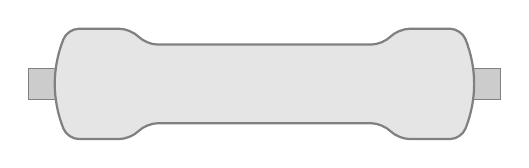
\begin{tikzpicture}
  % wire
  \draw[gray,fill=gray!40] (-3,-0.2) rectangle (3,0.2);
  % resistor
  \draw[rounded corners,thick,gray,fill=gray!20]
  ++(0,0.5) -- ++(1.5,0) -- ++(0.2,0.2) -- ++(0.8,0)
  .. controls +(0.2,-0.5) and +(0.2,0.5) .. ++(0,-1.4) -- ++(-0.8,0)
  -- ++(-0.2,0.2) -- ++(-3,0) -- ++(-0.2,-0.2) -- ++(-0.8,0)
  .. controls +(-0.2,0.5) and +(-0.2,-0.5) .. ++(0,1.4) -- ++(0.8,0)
  -- ++(0.2,-0.2) -- cycle;
  % band colors
  \stripe{-1.0}{brown}
  \stripe{0.0}{black}
  \stripe{1.0}{red}
  \Stripe{2.1}{gold!100!gray}
\end{tikzpicture}
\end{document}